\section{Machine Model}

% intro

% Our abstract machine model of a x86 multiprocessor system is illustrated in Figure \ref{fig:machine:overview}.

%We will start by defining an abstract machine model of a multiprocessor system that allows stores to be reordered after loads.
%Since we are only concerned with the machine's behaviour as observed by assembly programs, the internal structure of any real processor's microarchitecture is a highly abstracted.
%To keep the state space of the resulting model checking problems as small as possible, we defined our model on the basis of a 16 bit, 1 register machine.

% consistent with amd/intel litmus tests

% as observed by assembly programs.

% to reduce the state space, while emulating the behaviour of a x86 multiprocessor system.

% * abstract machine model to investigate the interaction of parallel programs through shared memory.

We will start by defining an abstract machine model of a multiprocessor system as observed by assembly programs.
To keep the state space of the resulting model checking problems as small as possible, it is based on a 16 bit architecture, using only a minimal set of registers and a radically reduced instruction set.

\begin{figure}[h]
  \centering
  % layers
\pgfdeclarelayer{background}
\pgfdeclarelayer{foreground}
\pgfsetlayers{background, main, foreground}

% styles
\tikzstyle{box} = [draw, text centered, rounded corners]
\tikzstyle{register} = [box, fill=white, minimum height=2em, minimum width=4em]
\tikzstyle{processor} = [draw, fill=blue!10, rounded corners]
\tikzstyle{buffer} = [processor, fill=red!10]%, dashed]

% distances
\def\blockdist{3}
\def\borderdist{0.2}

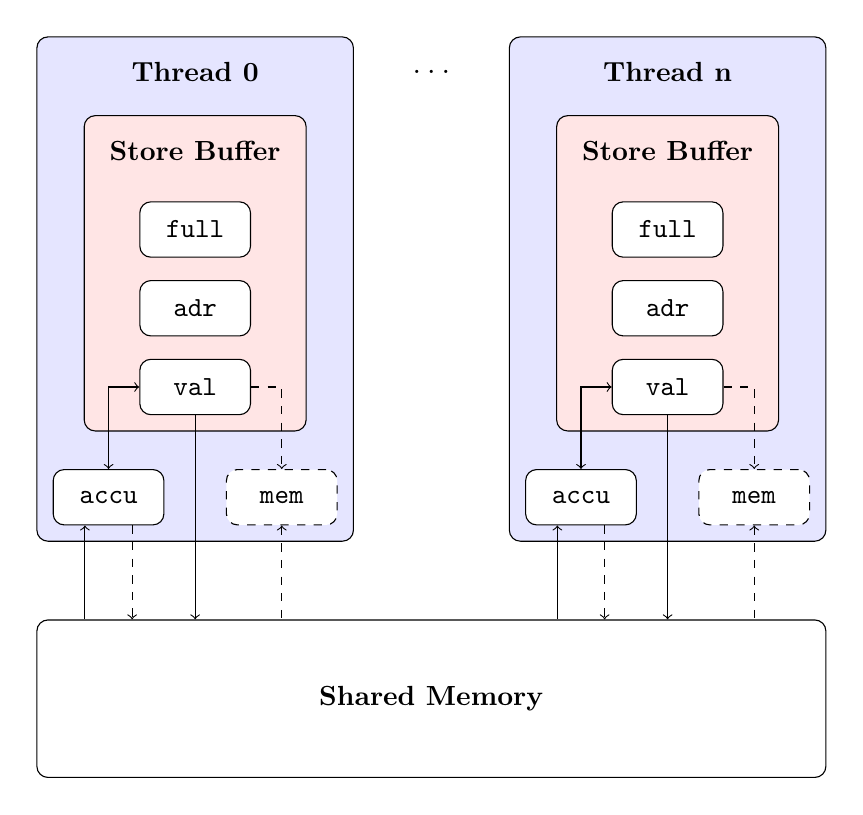
\begin{tikzpicture}

  % processor 0 %%%%%%%%%%%%%%%%%%%%%%%%%%%%%%%%%%%%%%%%%%%%%%%%%%%%%%%%%%%%%%%%
  \path (0, 0) node (title-0) [] {\textbf{Thread 0}};

  % store buffer
  \path (title-0)+(0, -1) node (sb-0) [] {\textbf{Store Buffer}};
  \path (sb-0)+(0, -1) node (full-0) [register] {\texttt{full}};
  \path (full-0)+(0, -1) node (adr-0) [register] {\texttt{adr}};
  \path (adr-0)+(0, -1) node (val-0) [register] {\texttt{val}};

  % registers
  \path (val-0)+(-1.1, -1.4) node (accu-0) [register] {\texttt{accu}};
  \path (val-0)+(1.1, -1.4) node (mem-0) [register, dashed] {\texttt{mem}};

  % paths
  \path [draw, <->] (val-0.west) -- (val-0.west -| accu-0.north) -- (accu-0.north);
  \path [draw, dashed, ->] (val-0.east) -- (val-0.east -| mem-0.north) -- (mem-0.north);

  \begin{pgfonlayer}{background}
    % bounding box
    \path (accu-0.west |- title-0.north)+(-\borderdist, \borderdist) node (a) {};
    \path (mem-0.south east)+(\borderdist, -\borderdist) node (b) {};
    \path [processor] (a) rectangle (b);

    % top left heap coordinate
    \path (a |- b)+(0, -1) node (tlh) {};

    % store buffer box
    \path (sb-0.north west)+(-\borderdist, \borderdist) node (a) {};
    \path (val-0.south -| sb-0.east)+(\borderdist, -\borderdist) node (b) {};
    \path [buffer] (a) rectangle (b);
  \end{pgfonlayer}

  % dots %%%%%%%%%%%%%%%%%%%%%%%%%%%%%%%%%%%%%%%%%%%%%%%%%%%%%%%%%%%%%%%%%%%%%%%
  \path (title-0)+(\blockdist, 0) node (dots) [] {\large $\ldots$};

  % processor n %%%%%%%%%%%%%%%%%%%%%%%%%%%%%%%%%%%%%%%%%%%%%%%%%%%%%%%%%%%%%%%%
  \path (dots)+(\blockdist, 0) node (title-n) [] {\textbf{Thread n}};

  % store buffer
  \path (title-n)+(0, -1) node (sb-n) [] {\textbf{Store Buffer}};
  \path (sb-n)+(0, -1) node (full-n) [register] {\texttt{full}};
  \path (full-n)+(0, -1) node (adr-n) [register] {\texttt{adr}};
  \path (adr-n)+(0, -1) node (val-n) [register] {\texttt{val}};

  % registers
  \path (val-n)+(-1.1, -1.4) node (accu-n) [register] {\texttt{accu}};
  \path (val-n)+(1.1, -1.4) node (mem-n) [register, dashed] {\texttt{mem}};

  % paths
  \path [draw, <->] (val-n.west) -- (val-n.west -| accu-n.north) -- (accu-n.north);
  \path [draw, dashed, ->] (val-n.east) -- (val-n.east -| mem-n.north) -- (mem-n.north);

  \begin{pgfonlayer}{background}
    % bounding box
    \path (accu-n.west |- title-n.north)+(-\borderdist, \borderdist) node (a) {};
    \path (mem-n.south east)+(\borderdist, -\borderdist) node (b) {};
    \path [processor] (a) rectangle (b);

    % bottom right heap coordinate
    \path (b)+(0, -\blockdist) node (brh) {};

    % store buffer box
    \path (sb-n.north west)+(-\borderdist, \borderdist) node (a) {};
    \path (val-n.south -| sb-n.east)+(\borderdist, -\borderdist) node (b) {};
    \path [buffer] (a) rectangle (b);
  \end{pgfonlayer}

  % heap %%%%%%%%%%%%%%%%%%%%%%%%%%%%%%%%%%%%%%%%%%%%%%%%%%%%%%%%%%%%%%%%%%%%%%%
  \path [box] (tlh) rectangle node (heap) [minimum height=2cm] {\textbf{Shared Memory}} (brh);

  % paths
  \path [draw, ->] (val-0) -- (heap.north -| val-0);
  \path [draw, <-, transform canvas={xshift=-3mm}] (accu-0) -- (heap.north -| accu-0);
  \path [draw, dashed, ->, transform canvas={xshift=3mm}] (accu-0) -- (heap.north -| accu-0);
  \path [draw, dashed, <-] (mem-0) -- (heap.north -| mem-0);

  \path [draw, ->] (val-n) -- (heap.north -| val-n);
  \path [draw, <-, transform canvas={xshift=-3mm}] (accu-n) -- (heap.north -| accu-n);
  \path [draw, dashed, ->, transform canvas={xshift=3mm}] (accu-n) -- (heap.north -| accu-n);
  \path [draw, dashed, <-] (mem-n) -- (heap.north -| mem-n);

\end{tikzpicture}

  \caption{Abstract Machine Model}
  \label{fig:machine:overview}
\end{figure}

A schematic overview is illustrated in Figure \ref{fig:machine:overview}.
At the top of the figure are an arbitrary number of processors, each containing:

\begin{itemize}
  \item \accu: a single 16 bit accumulator register
  \item \mem: a special purpose 16 bit register, storing the expected value required by a unary \emph{compare and swap} instruction
  % \item a \emph{store buffer} to break sequential consistency by delaying a single write, consisting of:
  \item a single element \emph{store buffer}, consisting of:
    \begin{itemize}
      \item \sbfull: a one bit flag register, signaling that it contains a value and may be flushed
      \item \sbadr: a 16 bit address register
      \item \sbval: a 16 bit value register
    \end{itemize}
\end{itemize}

All processors are directly connected to the machine's shared memory, referred to as \texttt{heap}, which will be uninitialized with the exception of any eventual input data.
In terms of memory ordering, the addition of a \emph{store buffer} allows stores to be reordered after loads, making our model consistent with Intel's or AMD's x86 memory ordering model \cite{intel, amd}.

\subsection{Instructions}

Our machine uses a radically reduced instruction set that contains only the most substantial operations.
Instructions are stored separately for each processor and are therefore not contained in memory.
This abstraction allows the program counter to address instructions by their index, starting from zero.
To simplify the definition of operational semantics, instructions are labelled using the following attributes:

\begin{itemize}
  \item \textbf{modify} -- Modifies a register's content.
  \item \textbf{read} -- Reads from memory using \emph{store forwarding}: if \sbfull{} is set and \sbadr{} equals the given target address, the value contained in \sbval{} is read instead of the corresponding shared memory location.
  \item \textbf{write} -- Writes to the store buffer by setting \sbfull{} to true, \sbadr{} to the given target address and \sbval{} to the value contained in \accu{}.
  \item \textbf{barrier} -- Blocks execution if the store buffer is full (\sbadr{} is set). %memory barrier% - requires the store buffer to be flushed
  \item \textbf{atomic} -- Multiple micro operations performed as a single, uninterruptible instruction.% (implies barrier)
  \item \textbf{control} -- Modifies the order in which instructions are executed.
\end{itemize}

Due to the single register architecture, all instructions have at most one operand.
Two addressing modes are supported, direct and indirect, denoted by square brackets (e.g. \texttt{LOAD [adr]}).

\newcommand{\defop}[3]{
  \paragraph{#1} \hfill #2
  \rule[0.5\baselineskip]{\textwidth}{0.1pt}\vspace{-0.5\baselineskip}\par\noindent
  #3
}

% \noindent
% \begin{tabu} to \textwidth {X[l]X[l]X[r]}
% \texttt{LOAD adr} & \texttt{accu = heap[adr]} & accu, read \\
% \texttt{STORE adr} & \texttt{heap[adr] = accu} & write
% \end{tabu}

\subsubsection{Memory}

\defop
{\texttt{LOAD adr}}
{accu, read}
{Loads the value found at address \texttt{adr} into \accu.}

\defop
{\texttt{STORE adr}}
{write}
{Stores the value found in \accu{} at address \texttt{adr}.}

\defop
{\texttt{FENCE}}
{barrier}
{Memory barrier.}

\subsubsection{Arithmetic}

\defop
{\texttt{ADD adr}}
{accu, read}
{Adds the value found at address \texttt{adr} to \accu.}

\defop
{\texttt{ADDI val}}
{accu}
{Adds the immediate value \texttt{val} to \accu.}

\defop
{\texttt{SUB adr}}
{accu, read}
{Subtracts the value found at address \texttt{adr} from \accu.}

\defop
{\texttt{SUBI val}}
{accu}
{Subtracts the immediate value \texttt{val} from \accu.}

\defop
{\texttt{MUL adr}}
{accu, read}
{Multiplies \accu{} with the value found at address \texttt{adr}.}

\defop
{\texttt{MULI val}}
{accu}
{Multiplies \accu{} with the immediate value \texttt{val}.}

\subsubsection{Control Flow}

\defop
{\texttt{CMP adr}}
{accu, read}
{Compares \accu{} to the value found at address \texttt{adr} by performing an unsigned subtraction.}

\defop
{\texttt{JMP pc}}
{control}
{Jumps to the statement at \texttt{pc} unconditionally.}

\defop
{\texttt{JZ pc}}
{control}
{Jumps to the statement at \texttt{pc} if \accu{} is zero.}

\defop
{\texttt{JNZ pc}}
{control}
{Jumps to the statement at \texttt{pc} if \accu{} is non-zero.}

\defop
{\texttt{JS pc}}
{control}
{Jumps to the statement at \texttt{pc} if \accu{} is negative (least significant bit is set).}

\defop
{\texttt{JNS pc}}
{control}
{Jumps to the statement at \texttt{pc} if \accu{} is zero or positive (least significant bit is unset).}

\defop
{\texttt{JNZNS pc}}
{control}
{Jumps to the statement at \texttt{pc} if \accu{} is positive (non-zero and least significant bit is unset).}

\subsubsection{Atomic}

\defop
{\texttt{MEM adr}}
{accu, mem, read}
{Loads the value found at address \texttt{adr} into \accu{} and \mem{} as the expectation during a latter \emph{compare and swap} operation.}

\defop
{\texttt{CAS adr}}
{accu, read, atomic, barrier}
{Atomically compares the expected value in \mem{} to the actual value found at address \texttt{adr} and only writes the value found in \accu{} back to address \texttt{adr} if they are equal.
Acts like a memory barrier.}

\subsubsection{Termination}

\defop
{\texttt{HALT}}
{barrier, control}
{Stops the current thread.}

\defop
{\texttt{EXIT val}}
{control}
{Stops the machine with exit code \texttt{val}.}

\subsubsection{Meta}

\defop
{\texttt{CHECK id}}
{control}
{Synchronize on checkpoint \texttt{id}.
Suspends execution until all threads, containing a call to checkpoint \texttt{id}, reached the corresponding \texttt{CHECK} statement.
This high-level meta instruction shall simplify the implementation of so called \emph{checker threads} used to validate machine states at runtime.}

\subsection{Programs}

Each processor is programmed using an assembly style language, defined by the following syntax.

\begin{figure}[h]
\begin{grammar}
\small

<int> ::= an integer number

<label> ::= a sequence of printable characters without "#"

<string> ::= a sequence of whitespace and printable characters without "#" and "\\n"

<comment> ::= "#" <string>

<nullary> ::= "FENCE" | "HALT"

<unary> ::= "ADDI" | "SUBI" | "MULI" | "EXIT" | "CHECK"

<memory> ::= "LOAD" | "STORE" | "ADD" | "SUB" | "MUL" | "CMP" | "MEM" | "CAS"

<jump> ::= "JMP" | "JZ" | "JNZ" | "JS" | "JNS" | "JNZNS"

<instruction> ::= <nullary>
\alt <unary> <int>
\alt <memory> ( <int> | "["<int>"]" )
\alt <jump> ( <int> | <label> )

<statement> ::= <label>":" <instruction> | <instruction>

<line> ::= <statement> | <statement> <comment> | <comment>

<program> ::= <line> | <line> "\\n" <program>
\end{grammar}
\caption{Program Syntax}
\label{fig:syntax:program}
\end{figure}

If the final statement in a given program is no control instruction, a final \texttt{HALT} is inserted implicitly.

\subsection{Scheduling}

At each step a processors either executes an instruction or flushes it's store buffer back to memory.
Scheduling is generally performed non-deterministically under the following constraints.

\begin{enumerate}
  \item A processor can execute a read, modify or control operation at any time.
  \item A processor can voluntarily flush its store buffer to memory only if it is full.
  \item A processor can execute a write, atomic or barrier operation only if it's store buffer is empty.
\end{enumerate}
